\chapter{METHODOLOGY}    

\section{MorphAI System Workflow Diagram}
      \begin{figure}[H]
        \centering
        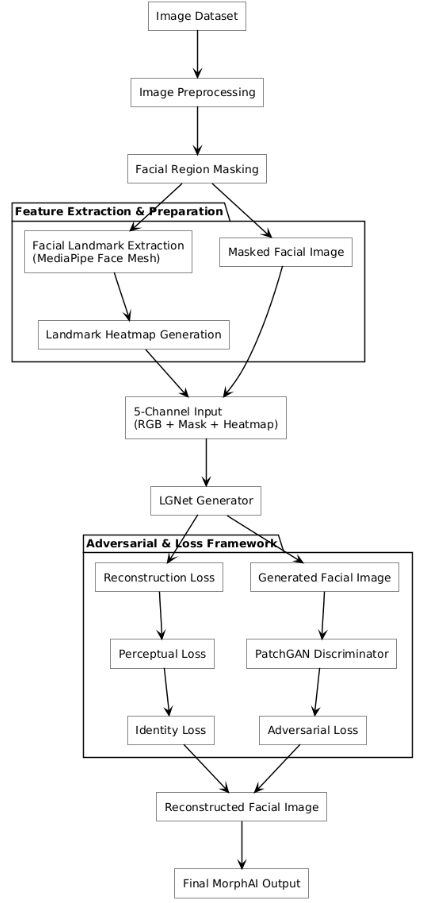
\includegraphics[scale=0.9]{img/model_arch.png}
        \caption{Stages of MorphAI System}
        \label{fig:blockdiagram}
    \end{figure}

\clearpage
\section{Description of Working Flow of the System}

The working process of MorphAI consists of several stages, starting from the input facial image and ending with the reconstructed facial image. The main stages of the system are described below.

\subsection{Image Dataset}

MorphAI uses facial images as the input dataset for training and evaluation. The original facial images are treated as ground-truth images. During training, different facial regions are masked so that the model learns to reconstruct the missing regions.

\subsection{Image Preprocessing}

The input images are resized and converted into a suitable format for the model. Facial landmark detection is then performed on the processed images to obtain the structural information required by the reconstruction system.

\subsection{Facial Region Masking}

A facial region is selected for reconstruction using a binary mask. The mask identifies the area that will be removed or hidden from the input image. MorphAI supports facial regions such as the eyes, eyebrows, nose, and mouth.

\subsection{Feature Extraction and Preparation}

After masking, the system prepares the information required by the reconstruction model. MediaPipe Face Mesh is used to extract facial landmarks from the input image.

\noindent The detected landmarks are then used to generate a landmark heatmap. The heatmap provides additional information about the position and structure of facial features.

\noindent At the same time, the masked facial image is prepared as a separate input. These components are then combined to form the model input.

\clearpage
\subsection{Five-Channel Input Formation}

MorphAI combines the RGB image, facial mask, and landmark heatmap to create a five-channel input:
\begin{equation}
3\text{ RGB channels} + 1\text{ mask channel} + 1\text{ heatmap channel}
= 5\text{ channels}.
\end{equation}

\noindent The resulting input has the form:

\begin{equation}
X \in \mathbb{R}^{5 \times 256 \times 256}.
\end{equation}

\noindent This allows the generator to use both visual information and facial structural information during reconstruction.

\subsection{LGNet Generator}

The five-channel input is passed to the modified LGNet generator. The generator uses the visible facial information, mask, and landmark heatmap to reconstruct the missing facial region.

\noindent The output of the generator is a generated facial image containing the reconstructed region.

\subsubsection{Loss Framework}
The generated image is optimized using a composite loss framework during
training. The loss function combines reconstruction, perceptual, style,
identity, facial landmark, and adversarial losses to guide the generator
toward accurate reconstruction, preservation of facial structure, texture
consistency, identity preservation, and visual realism. The individual
loss terms are defined, and the total
training objective is given by:

\begin{equation}
\mathcal{L}_{\text{total}} = \lambda_{1}\mathcal{L}_{\text{L1}} +
\lambda_{\text{perc}}\mathcal{L}_{\text{perceptual}} +
\lambda_{\text{style}}\mathcal{L}_{\text{style}} +
\lambda_{\text{id}}\mathcal{L}_{\text{identity}} +
\lambda_{\text{lm}}\mathcal{L}_{\text{landmark}} +
\lambda_{\text{adv}}\mathcal{L}_{\text{adv}}
\label{eq:total-loss}
\end{equation}

\noindent where $\lambda_{1}$, $\lambda_{\text{perc}}$, $\lambda_{\text{style}}$,
$\lambda_{\text{id}}$, $\lambda_{\text{lm}}$, and $\lambda_{\text{adv}}$
are the weighting coefficients for each loss term.

\subsection{Reconstructed Facial Image}

After the generator and loss-based optimization, the reconstructed facial image is obtained. The generated region is combined with the remaining facial region to produce a complete reconstructed face.

\clearpage
\subsubsection{Final MorphAI Output}
The final output of MorphAI is the reconstructed facial image. The output is
intended to preserve the facial structure, appearance, and identity of the input
image while reconstructing the selected facial region.

\section{Model Architecture}

% \begin{figure}[H]
%     \centering
%     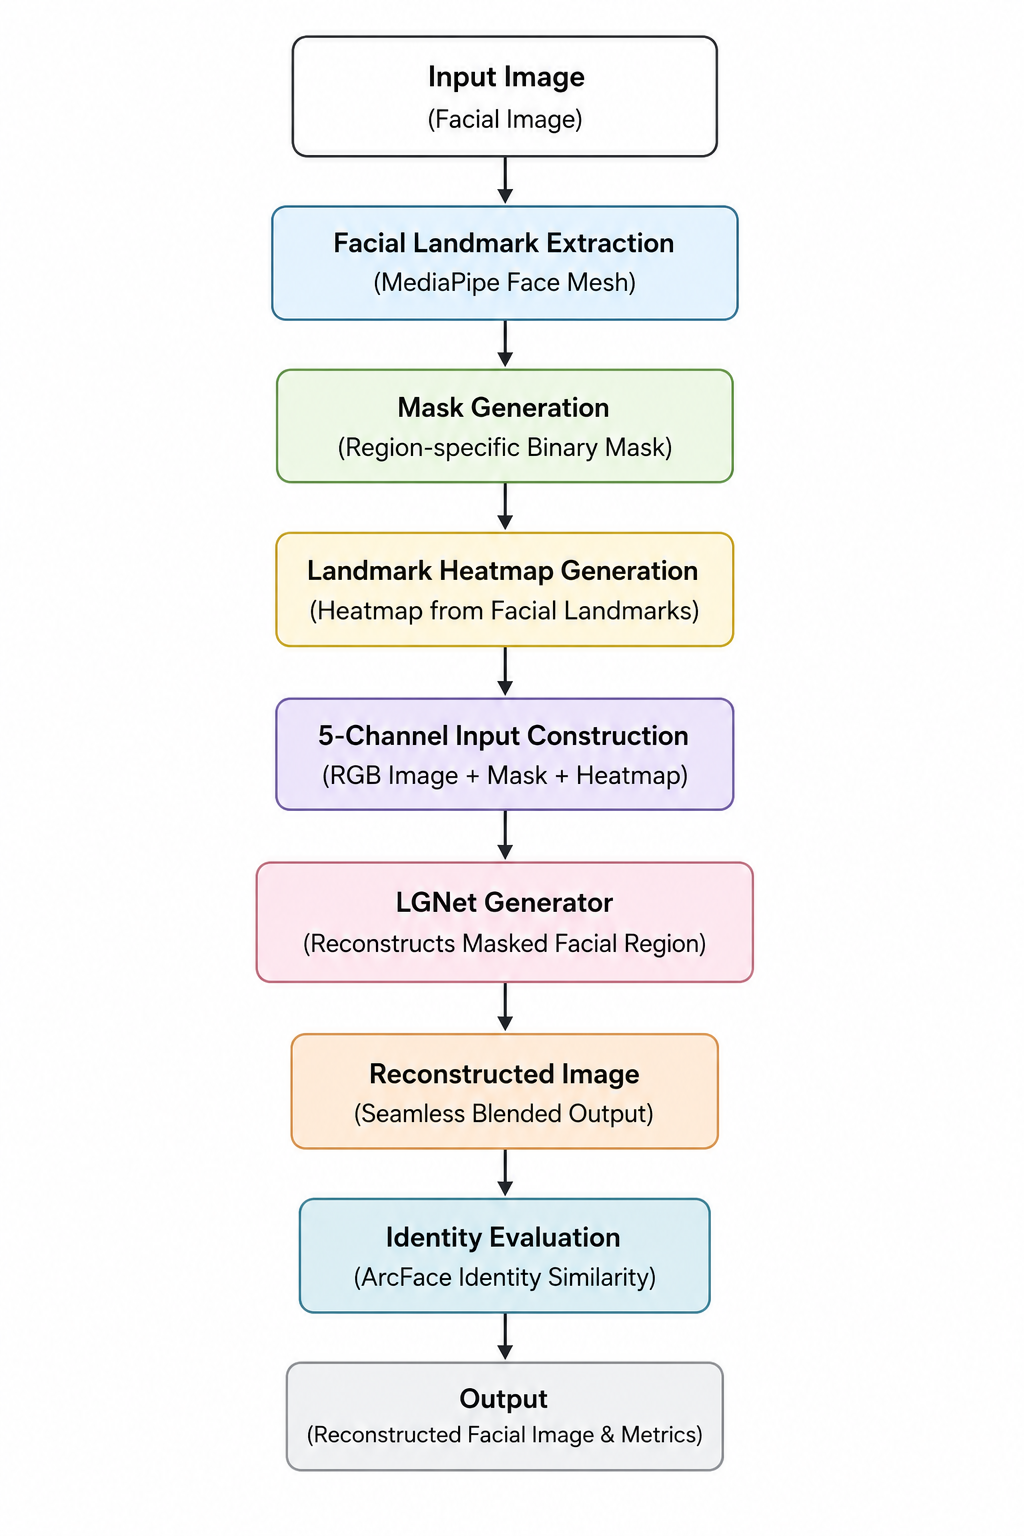
\includegraphics[width=0.85\textwidth]{img/morphai_architecture.png}
%     \caption{MorphAI model architecture}
%     \label{fig:morphai_architecture}
% \end{figure}

\begin{figure}[htbp]
    \centering
    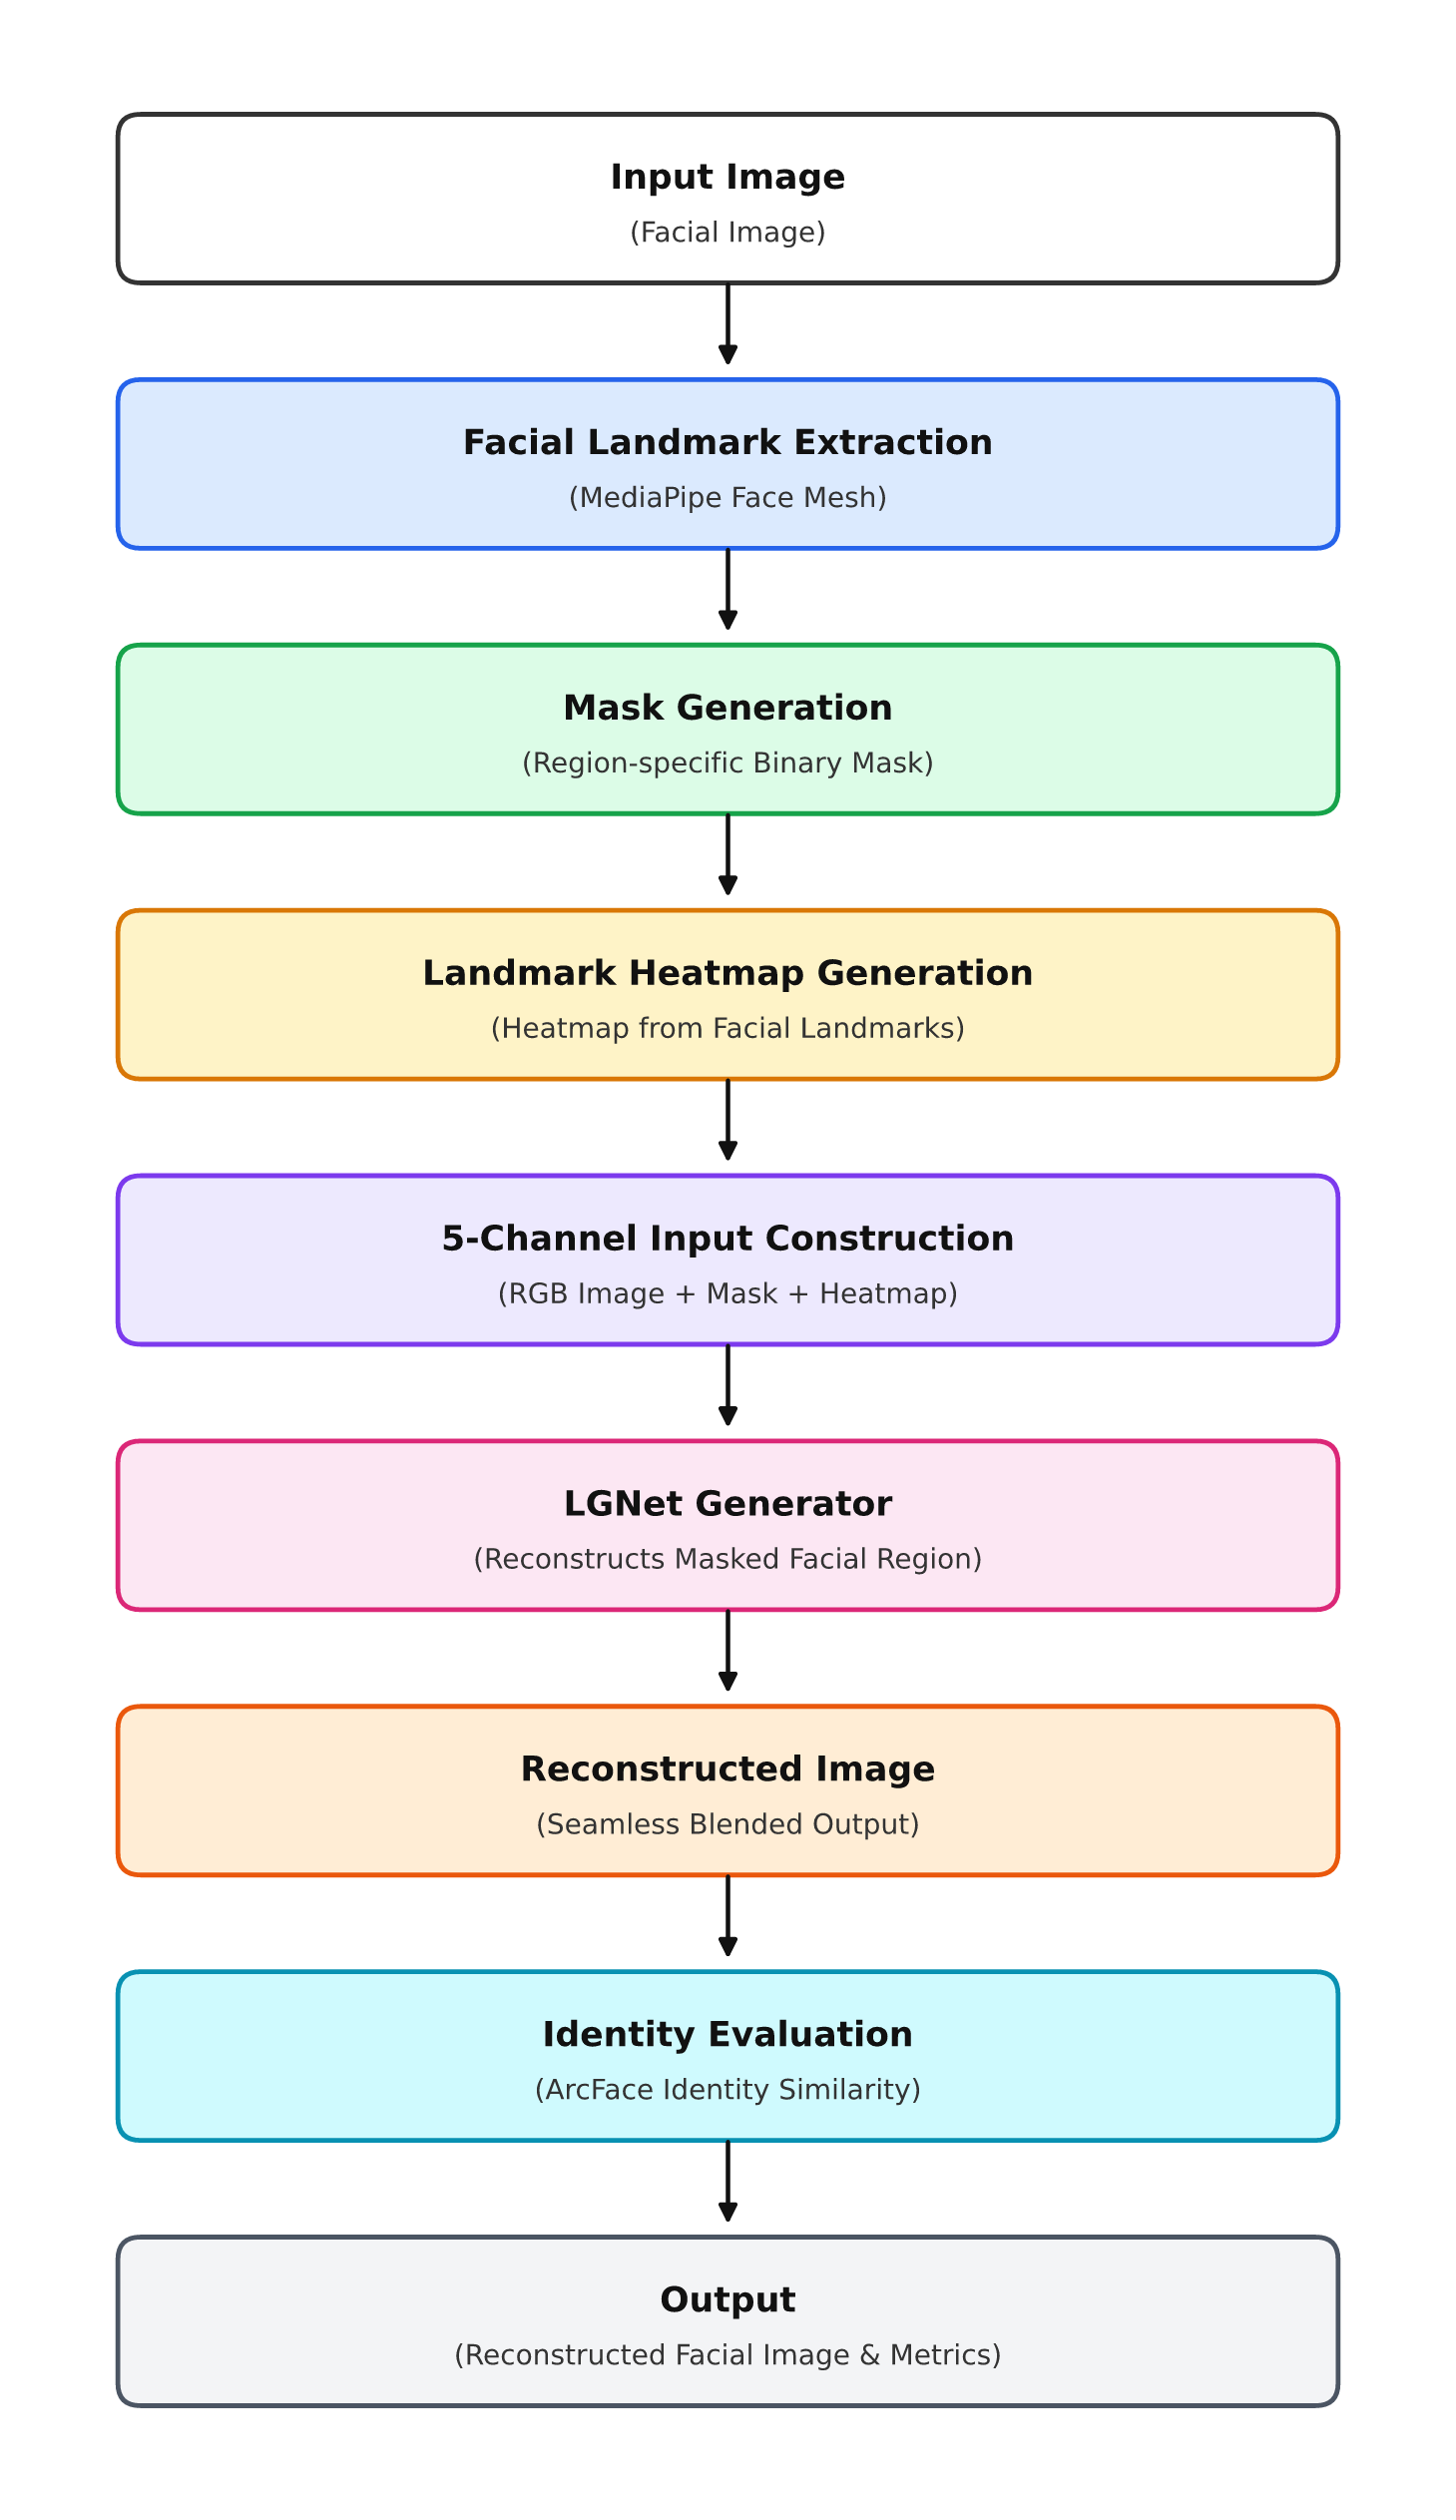
\includegraphics[width=0.85\textwidth]{img/fig3_2_clean.png}
    \caption{MorphAI model architecture}
    \label{fig:morphai_architecture}
\end{figure}

\noindent MorphAI adopts a facial inpainting architecture designed to reconstruct
selected facial regions while preserving the overall appearance and
identity of the input face. The system combines facial landmark
extraction, mask generation, landmark-based guidance, and the LGNet
generator to produce the reconstructed image.

% \begin{figure}[H]
%     \centering
%     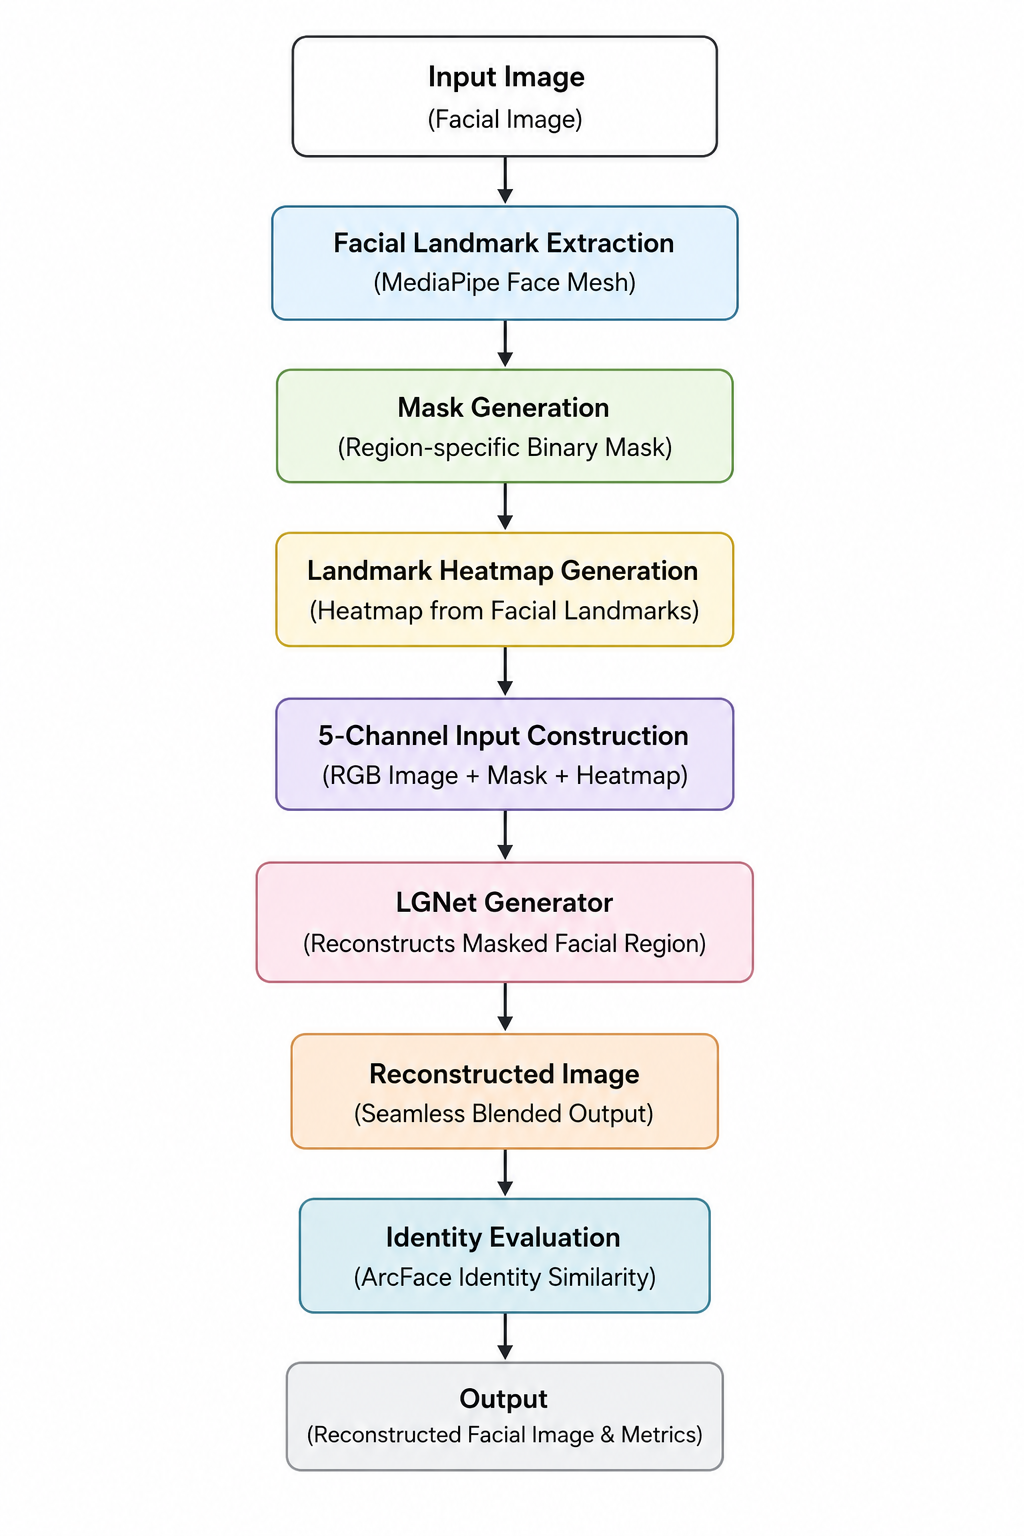
\includegraphics[width=0.85\textwidth]{img/morphai_architecture.png}
%     \caption{MorphAI model architecture}
%     \label{fig:morphai_architecture}
% \end{figure}

\subsection{Input Image}

The system receives a facial image from the user through the frontend.
The image is prepared and passed to the backend for facial region
selection and reconstruction.

\subsection{Facial Landmark Extraction}

The LandmarkExtractor detects important facial landmarks from the input
image. These landmarks provide structural information about the face
and help guide the reconstruction of the selected region.

\subsection{Mask Generation}

The MaskGenerator creates a region-specific binary mask based on the
selected facial area. The mask identifies the region to be reconstructed
while preserving the remaining facial content.

\subsection{Landmark Heatmap}

The detected landmarks are converted into a spatial heatmap. This
heatmap provides the generator with additional information about the
facial structure and location of important facial features.

\clearpage
\subsection{LGNet Generator}

The LGNetGenerator is the main reconstruction component of MorphAI. It
receives the RGB image, facial mask, and landmark-based information as
the required multi-channel input. The generator processes these inputs
and reconstructs the selected facial region while maintaining
consistency with the surrounding facial features.

\subsection{Identity Evaluation}

The reconstructed image can be evaluated using the IdentityExtractor
to determine whether the generated face maintains the identity
characteristics of the original input. This provides an additional
measure for assessing the quality of the reconstruction.

% \begin{figure}[htbp]
%     \centering
%     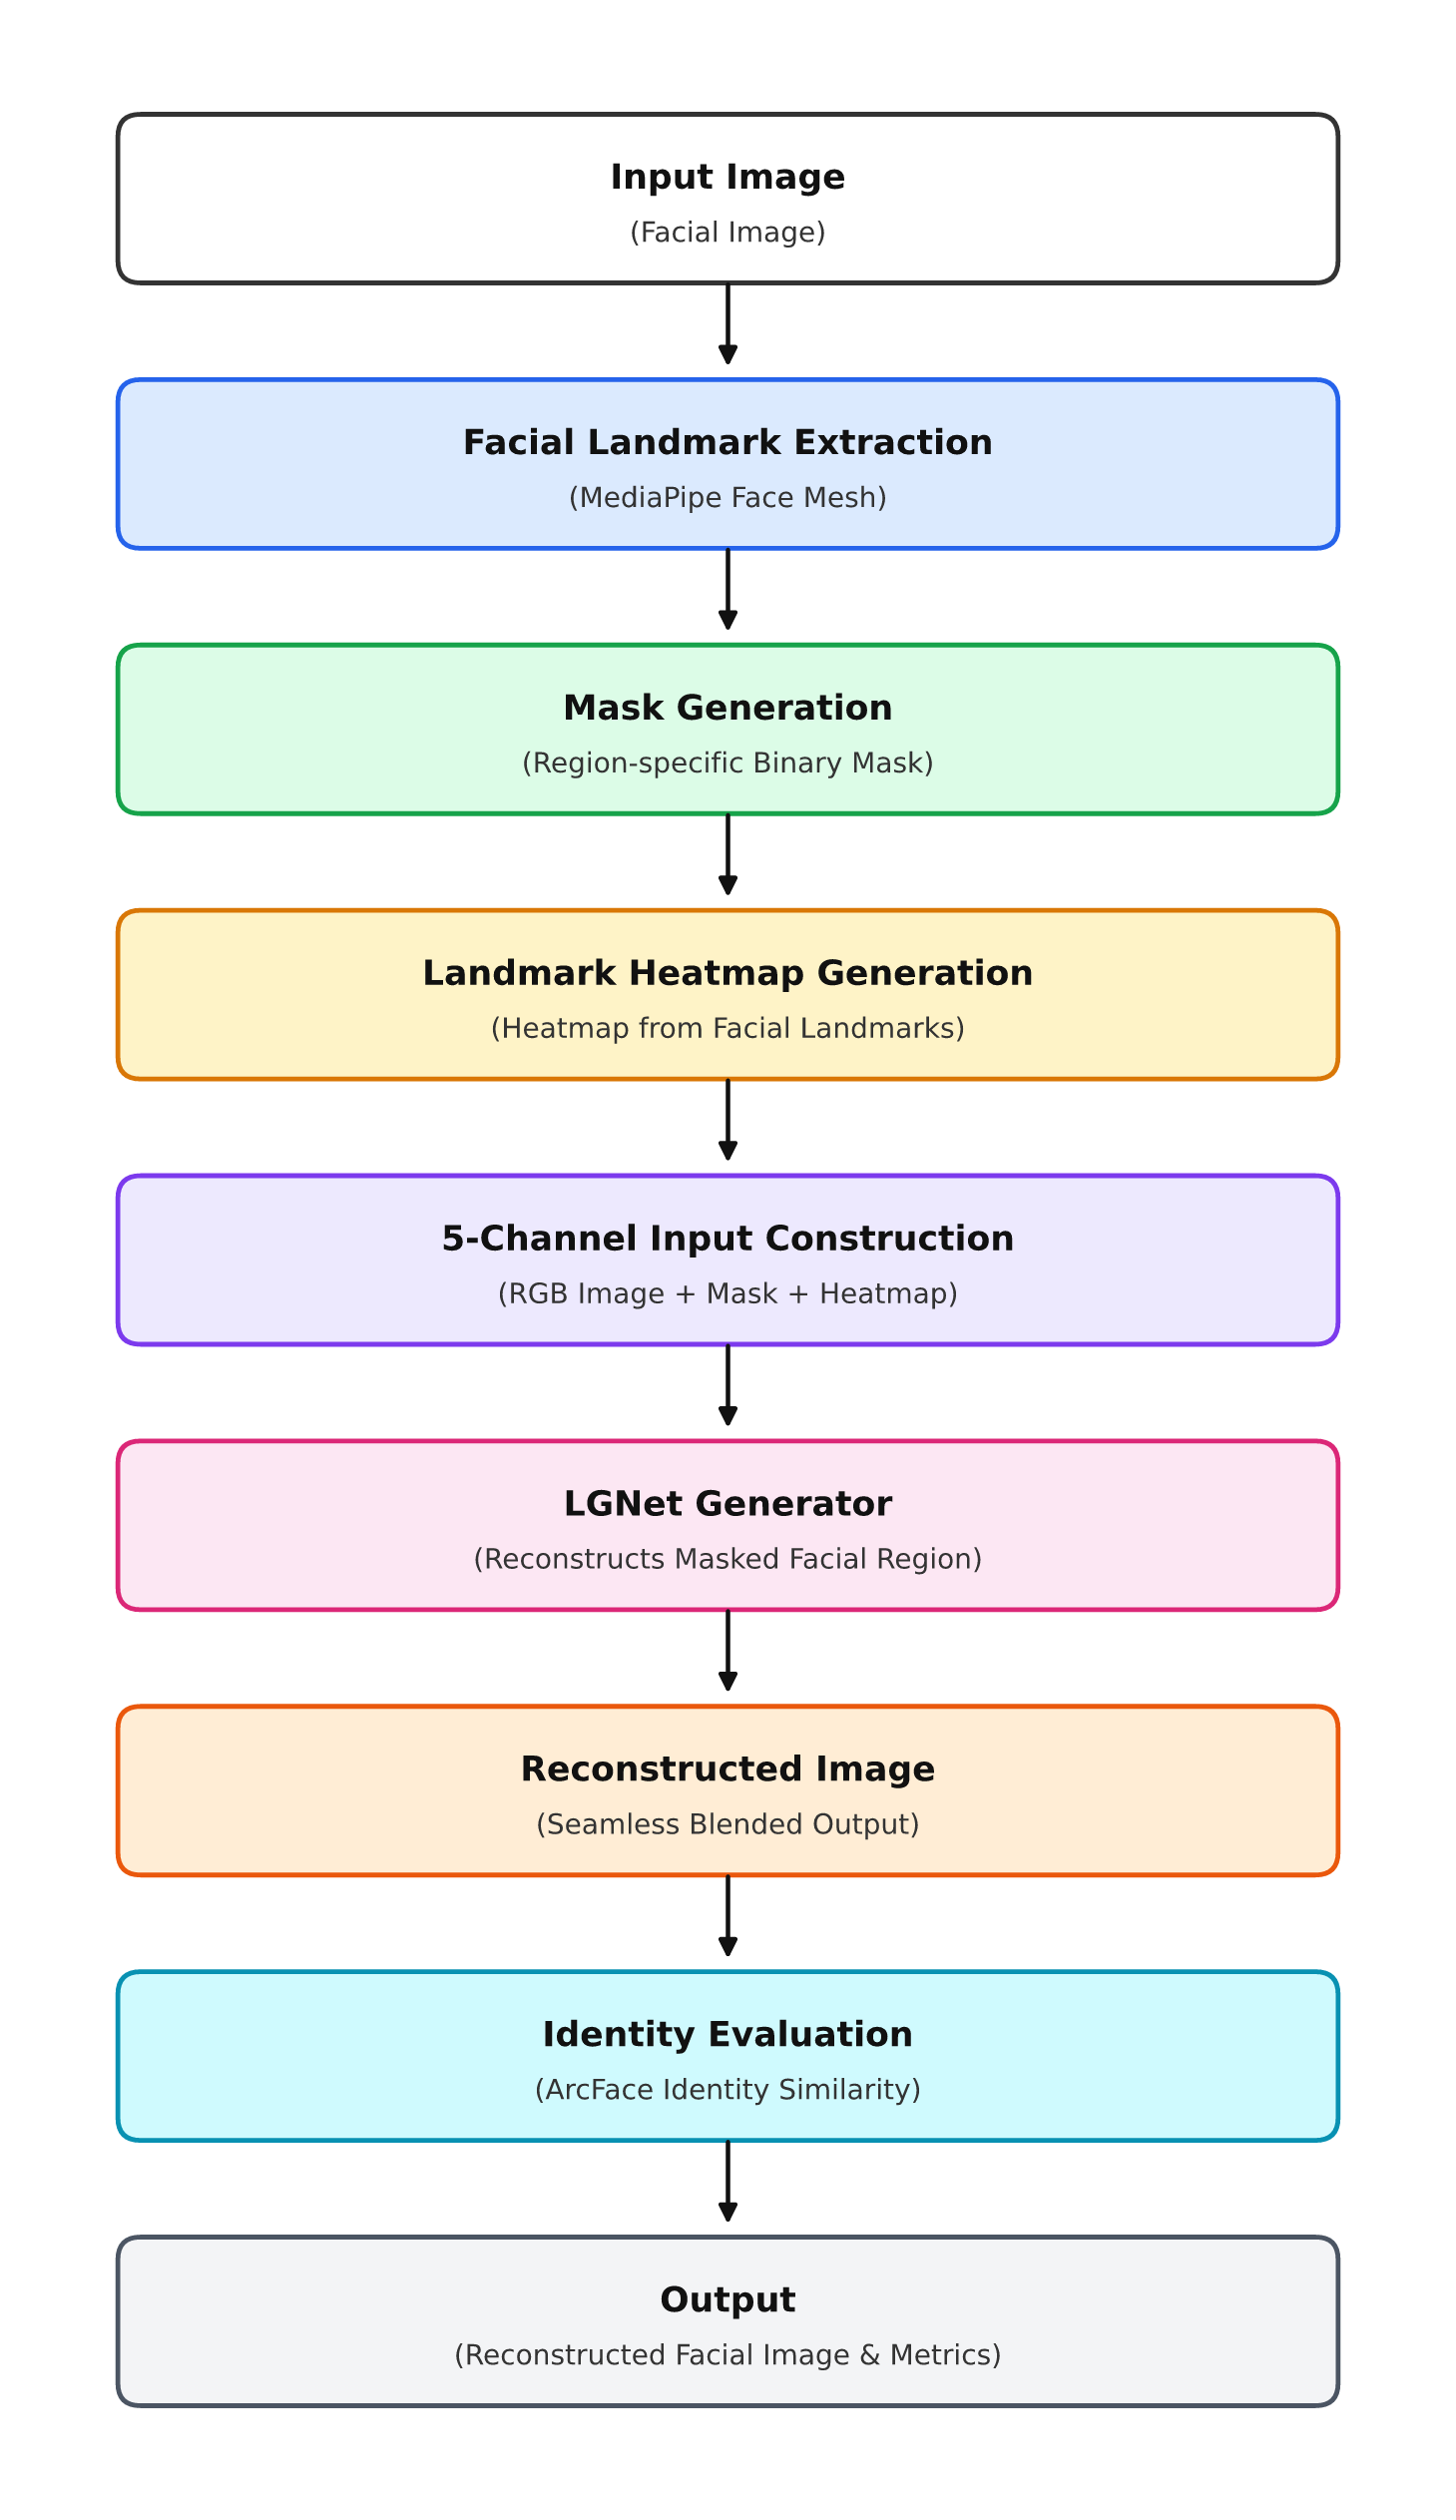
\includegraphics[width=0.85\textwidth]{img/fig3_2_clean.png}
%     \caption{MorphAI model architecture}
%     \label{fig:morphai_architecture}
% \end{figure}


% \clearpage
\subsection{Model Architecture Summary}

Table~\ref{tab:morphai_arch} summarises the main components of the
MorphAI architecture.

\begin{table}[H]
\centering
\caption{MorphAI model architecture summary}
\label{tab:morphai_arch}
\begin{tabular}{ll}
\hline
\textbf{Component} & \textbf{Purpose} \\
\hline
Frontend & Image upload and region selection \\
LandmarkExtractor & Detect facial landmarks \\
MaskGenerator & Generate the reconstruction mask \\
Landmark Heatmap & Provide facial structural guidance \\
LGNetGenerator & Reconstruct the selected facial region \\
IdentityExtractor & Evaluate identity preservation \\
\hline
\end{tabular}
\end{table}
% ────────────────────────────────────────────────────────────────────

\subsection{Technical Contribution of MorphAI}
The primary technical contribution of MorphAI is the incorporation of explicit facial 
landmark heatmap conditioning into a modified LGNet-based facial inpainting framework. Rather than introducing an entirely new generative architecture, MorphAI builds on the existing Local-Global Network (LGNet) generator and extends it with structural guidance 
derived from facial landmarks.

\noindent The model receives a five-channel input consisting of the RGB facial image (3 channels), 
a binary facial mask (1 channel), and a landmark heatmap (1 channel):
\begin{equation}
    X = [I_{RGB}, M, H] \in \mathbb{R}^{5 \times 256 \times 256}
\end{equation}

\noindent The landmark heatmap $H$ provides the generator with explicit spatial information about the position and shape of important facial features, which is not available to the 
original LGNet or to context-only inpainting models such as LaMa. This allows the 
generator to combine two complementary sources of information during reconstruction: 
the visual context surrounding the masked region, and the underlying facial geometry 
indicated by the landmarks.

\noindent In addition to landmark conditioning, MorphAI incorporates identity-preserving supervision using ArcFace-based facial embeddings during training, encouraging the reconstructed 
region to remain consistent with the identity of the input subject. This distinguishes MorphAI from landmark-based methods such asDeepFaceReshaping~\cite{chen2024deepface}, 
which use landmarks primarily to drive interactive geometric reshaping of \textit{visible} 
facial regions, rather than as a conditioning signal for reconstructing \textit{missing} 
regions.

\noindent Overall, the novelty of MorphAI lies in the combination of the following elements, 
rather than in proposing a new generative architecture:
\begin{enumerate}
    \item Landmark heatmap conditioning,
    \item Identity-preserving loss supervision, and
    \item Application of this combined approach to region-specific facial inpainting.
\end{enumerate}
MorphAI is therefore best described as a landmark-conditioned, identity-preserving 
adaptation of LGNet for facial region reconstruction.


\section{Hyperparameters}

The MorphAI model was trained using PyTorch with Automatic Mixed Precision
(autocast). The training configuration was selected to balance reconstruction
quality, facial structure, texture consistency, and identity preservation.

\begin{itemize}
    \item \textbf{Training Configuration:} The MorphAI model was trained for 5 epochs using the CelebA-HQ dataset containing 16,800 facial images. A portion of these images was held out for evaluation.
    
    \item \textbf{Loss Function:} A composite loss combining L1, perceptual,
    style, identity, and facial landmark losses was used to improve
    reconstruction quality and preserve facial characteristics.
    
    \item \textbf{L1 Loss:} Measures pixel-level differences between the
    reconstructed and target images.
    
    \item \textbf{Perceptual Loss:} Uses VGG-16 features to preserve important
    facial structures and visual details.
    
    \item \textbf{Style Loss:} Uses Gram matrix features to maintain texture
    and appearance consistency.
    
    \item \textbf{Identity Loss:} Uses facial embedding cosine similarity to
    preserve the identity of the input subject.
    
    \item \textbf{Landmark Loss:} Uses Wing loss to maintain the position and
    structure of important facial landmarks.

    \item \textbf{Adversarial Loss:} Uses a PatchGAN discriminator trained
jointly with the generator to improve the local realism and texture
fidelity of reconstructed facial regions.
    
    \item \textbf{Training Efficiency:} Automatic Mixed Precision was used
    to reduce GPU memory consumption and improve training efficiency.
    
    \item \textbf{Training Convergence:} Training loss decreased from
    0.3479 in the first epoch to 0.2774 in the fifth epoch, while validation
    loss decreased from 0.3640 to 0.2950, indicating stable convergence.
    
    \item \textbf{Final Checkpoint:} The fifth-epoch checkpoint,
    \texttt{morphai\_epoch\_05.pt}, was selected as the final model for
    evaluation and comparison with the LaMa baseline.
\end{itemize}

% \noindent Table~\ref{tab:hparams} summarizes the main training configuration.

\begin{table}[H]
\centering
\caption{Training configuration of the proposed LGNet model}
\label{tab:hparams}
\renewcommand{\arraystretch}{1.3}
\begin{tabular}{|l|l|}
\hline
\textbf{Training Setting} & \textbf{Value} \\ \hline
Framework & PyTorch \\ \hline
Training method & Automatic Mixed Precision (autocast) \\ \hline
Training epochs & 5 \\ \hline
% Dataset size & 28,000 facial images \\ \hline
Dataset & CelebA-HQ (16,800 facial images) \\ \hline
Loss function & Composite multi-objective loss \\ \hline
Pixel loss & L1 loss \\ \hline
Perceptual loss & VGG-16 based \\ \hline
Style loss & Gram matrix based \\ \hline
Adversarial loss    PatchGAN discriminator\\ \hline
Identity loss & Face embedding cosine loss \\ \hline
Landmark loss & Wing loss \\ \hline
Final checkpoint & \texttt{morphai\_epoch\_05.pt} \\ \hline
\end{tabular}
\end{table}

\section{Performance Evaluation Metrics}

MorphAI is evaluated using metrics that measure reconstruction quality,
visual similarity, and identity preservation. The evaluation was performed
using 2,800 held-out facial images. For each held-out image, six
facial-region masks were generated for the left eyebrow, right eyebrow,
left eye, right eye, nose, and mouth. Therefore, the evaluation consisted
of $2,800 \times 6 = 16,800$ region-specific evaluation samples. These
16,800 samples are derived evaluation instances and do not represent
16,800 unique facial images.

\subsection{Peak Signal-to-Noise Ratio (PSNR)}

PSNR measures the pixel-level similarity between the reconstructed image and the original image. A higher PSNR value indicates that the reconstructed image is closer to the ground-truth image.

\begin{equation}
\text{PSNR} =
10\log_{10}\left(\frac{MAX_I^2}{\text{MSE}}\right)
\end{equation}

\noindent where $MAX_I$ is the maximum possible pixel value and MSE is the mean squared error.

\subsection{Structural Similarity Index (SSIM)}

SSIM measures how similar the structure of the reconstructed image is to the original image. It considers factors such as brightness, contrast, and structural information. Higher SSIM indicates better structural similarity.

\subsection{Learned Perceptual Image Patch Similarity (LPIPS)}

LPIPS measures perceptual similarity using features extracted from a deep neural network. It is useful for checking whether the reconstructed facial region looks visually similar to the original. Lower LPIPS values indicate better perceptual similarity.

\subsection{Fréchet Inception Distance (FID)}

FID compares the feature distributions of generated and real images. It is mainly used to measure the realism of generated images. A lower FID value indicates that the generated images are closer to real facial images.

\subsection{Identity Similarity}

Identity similarity measures whether the reconstructed face still represents the same person as the original image. MorphAI uses facial embeddings and cosine similarity for this evaluation.

\begin{equation}
\text{Identity Similarity} =
\frac{f(\hat{I}) \cdot f(I)}
{\|f(\hat{I})\|_2 \|f(I)\|_2}
\end{equation}

\noindent where $f(I)$ and $f(\hat{I})$ represent the facial embeddings of the original and reconstructed images, respectively. Higher similarity indicates better identity preservation.

\subsection{Root Mean Square Error (RMSE)}

RMSE measures the average pixel-level difference between the reconstructed image and the ground-truth image. Lower RMSE indicates smaller reconstruction errors.

\begin{equation}
\text{RMSE} =
\sqrt{
\frac{1}{CHW}
\sum_{c=1}^{C}
\sum_{h=1}^{H}
\sum_{w=1}^{W}
\left(\hat{I}_{c,h,w}-I_{c,h,w}\right)^2
}
\end{equation}

\noindent where $\hat{I}$ is the reconstructed image and $I$ is the ground-truth image.

\subsection{RMSE-log}

RMSE-log measures the reconstruction error after applying a logarithmic
transformation to the pixel values. It reduces the influence of large
pixel differences and provides an error measure on a logarithmic scale.

\noindent The RMSE-log is defined as:

\label{sec:rmse-log}
\begin{equation}
RMSE_{\log} =
\sqrt{
\frac{1}{CHW}
\sum_{c=1}^{C}
\sum_{h=1}^{H}
\sum_{w=1}^{W}
\left[
\log(1+\hat{I}_{c,h,w})
-
\log(1+I_{c,h,w})
\right]^2
}
\label{eq:rmse-log}
\end{equation}

\noindent where $I$ represents the ground-truth image, $\hat{I}$ represents the
reconstructed image, $C$ is the number of image channels, and $H$ and
$W$ are the image height and width, respectively. The $\log(1+x)$
transformation allows zero-valued pixels to be handled safely.

\noindent Lower RMSE-log values indicate smaller reconstruction errors and
therefore better reconstruction quality.
 
\section{Model Variants Explored}

Different inpainting configurations were evaluated during the development
of MorphAI. LaMa was used as a pretrained baseline, while LGNet was used
as the main inpainting model. A modified LGNet configuration was then
developed by providing RGB images together with a binary facial mask and
landmark heatmap. The main variants are summarized in
Table~\ref{tab:model_variants_ch3}, while their quantitative results are
presented in Section~5.1.

\begin{table}[h!]
\centering
\renewcommand{\arraystretch}{1.4}
\begin{tabular}{|l|p{9cm}|}
\hline
\textbf{Variant} & \textbf{Description} \\ \hline

LaMa & Pretrained image inpainting model. \\ \hline

LGNet & Inpainting model used for facial reconstruction. \\ \hline

\textbf{LGNet + 5-channel input} &
\textbf{Modified LGNet using RGB image, binary facial mask, and landmark
heatmap for guided facial reconstruction.} \\ \hline

\end{tabular}
\caption{Model variants explored during MorphAI development}
\label{tab:model_variants_ch3}
\end{table}